        %% Преамбула TeX-файла

% 1. Стиль и язык
\documentclass[utf8x]{G7-32} % Стиль (по умолчанию будет 14pt)
\usepackage[T2A]{fontenc}
\usepackage[russian]{babel}

% Остальные стандартные настройки убраны в preamble.inc.tex.

\usepackage{booktabs}
\usepackage{pdflscape}
\usepackage{longtable}
\usepackage{pdflscape}
\usepackage{lscape}
\usepackage{cancel}
% Настройки листингов.
% 8 Листинги

\usepackage{listings}

% Значения по умолчанию
\lstset{
  basicstyle= \footnotesize,
  breakatwhitespace=true,% разрыв строк только на whitespacce
  breaklines=true,       % переносить длинные строки
%   captionpos=b,          % подписи снизу -- вроде не надо
  inputencoding=koi8-r,
  numbers=left,          % нумерация слева
  numberstyle=\footnotesize,
  showspaces=false,      % показывать пробелы подчеркиваниями -- идиотизм 70-х годов
  showstringspaces=false,
  showtabs=false,        % и табы тоже
  stepnumber=1,
  tabsize=4,              % кому нужны табы по 8 символов?
  frame=single
}

% Стиль для псевдокода: строчки обычно короткие, поэтому размер шрифта побольше
\lstdefinestyle{pseudocode}{
  basicstyle=\small,
  keywordstyle=\color{black}\bfseries\underbar,
  language=Pseudocode,
  numberstyle=\footnotesize,
  commentstyle=\footnotesize\it
}

% Стиль для обычного кода: маленький шрифт
\lstdefinestyle{realcode}{
  basicstyle=\scriptsize,
  numberstyle=\footnotesize
}

% Стиль для коротких кусков обычного кода: средний шрифт
\lstdefinestyle{simplecode}{
  basicstyle=\footnotesize,
  numberstyle=\footnotesize
}

% Стиль для BNF
\lstdefinestyle{grammar}{
  basicstyle=\footnotesize,
  numberstyle=\footnotesize,
  stringstyle=\bfseries\ttfamily,
  language=BNF
}

% Определим свой язык для написания псевдокодов на основе Python
\lstdefinelanguage[]{Pseudocode}[]{Python}{
  morekeywords={each,empty,wait,do},% ключевые слова добавлять сюда
  morecomment=[s]{\{}{\}},% комменты {а-ля Pascal} смотрятся нагляднее
  literate=% а сюда добавлять операторы, которые хотите отображать как мат. символы
    {->}{\ensuremath{$\rightarrow$}~}2%
    {<-}{\ensuremath{$\leftarrow$}~}2%
    {:=}{\ensuremath{$\leftarrow$}~}2%
    {<--}{\ensuremath{$\Longleftarrow$}~}2%
}[keywords,comments]

% Свой язык для задания грамматик в BNF
\lstdefinelanguage[]{BNF}[]{}{
  morekeywords={},
  morecomment=[s]{@}{@},
  morestring=[b]",%
  literate=%
    {->}{\ensuremath{$\rightarrow$}~}2%
    {*}{\ensuremath{$^*$}~}2%
    {+}{\ensuremath{$^+$}~}2%
    {|}{\ensuremath{$|$}~}2%
}[keywords,comments,strings]

% Подписи к листингам на русском языке.
\renewcommand\lstlistingname{\cyr\CYRL\cyri\cyrs\cyrt\cyri\cyrn\cyrg}
\renewcommand\lstlistlistingname{\cyr\CYRL\cyri\cyrs\cyrt\cyri\cyrn\cyrg\cyri}

\sloppy

% Настройки стиля ГОСТ 7-32
% Для начала определяем, хотим мы или нет, чтобы рисунки и таблицы нумеровались в пределах раздела, или нам нужна сквозная нумерация.
\EqInChapter % формулы будут нумероваться в пределах раздела
\TableInChapter % таблицы будут нумероваться в пределах раздела
\PicInChapter % рисунки будут нумероваться в пределах раздела

% Добавляем гипертекстовое оглавление в PDF
\usepackage[
bookmarks=true, colorlinks=true, unicode=true,
urlcolor=black,linkcolor=black, anchorcolor=black,
citecolor=black, menucolor=black, filecolor=black,
]{hyperref}

% Изменение начертания шрифта --- после чего выглядит таймсоподобно.
% apt-get install scalable-cyrfonts-tex

\IfFileExists{cyrtimes.sty}
    {
        \usepackage{cyrtimespatched}
    }
    {
        % А если Times нету, то будет CM...
    }

\usepackage{graphicx}   % Пакет для включения рисунков

% С такими оно полями оно работает по-умолчанию:
% \RequirePackage[left=20mm,right=10mm,top=20mm,bottom=20mm,headsep=0pt]{geometry}
% Если вас тошнит от поля в 10мм --- увеличивайте до 20-ти, ну и про переплёт не забывайте:
\geometry{right=20mm}
\geometry{left=30mm}


% Пакет Tikz
\usepackage{tikz}
\usetikzlibrary{arrows,positioning,shadows}

% Произвольная нумерация списков.
\usepackage{enumerate}

% ячейки в несколько строчек
\usepackage{multirow}

% itemize внутри tabular
\usepackage{paralist,array}
\usepackage{longtable}
% Любимые команды
\newcommand{\Code}[1]{\textbf{#1}}

% Полезные макросы листингов.


\title{Курсовая  работа}
\author{}
 

\begin{document}


%Изменим нумерацию на более привычную...
%... и нарушим этим гост.

\renewcommand{\labelenumi}{\arabic{enumi})}
\renewcommand{\labelenumii}{\asbuk{enumii})}


\frontmatter % выключает нумерацию ВСЕГО; здесь начинаются ненумерованные главы: реферат, введение, глоссарий, сокращения и прочее.

% Команды \breakingbeforechapters и \nonbreakingbeforechapters
% управляют разрывом страницы перед главами.
% По-умолчанию страница разрывается.

% \nobreakingbeforechapters
% \breakingbeforechapters


\pagestyle{empty} % нумерация выкл.

\begin{center}
    \textup{Высшая школа экономики \\Факультет компьютерных наук}
\\[20mm]
     
%    \includegraphics[width=50mm]{msu.eps}
 
       \textup{\large\bfseries
         \\[10mm]Разработка алгоритма управления длиннофокусной камерой для распознавания людей в публичных пространствах \\Построение оптимального пути для обхода длиннофокусной камерой множества движущихся объектов\\[15pt]
         Курсовая работа  \\[15pt]
Хайбрахманов Тимур Радикович  \\
Тимченко Даниил Геннадьевич   }\\[30mm]

\begin{tabular}{l}
  \\
 \\[25pt]
\end{tabular}




    \begin{tabular}{p{250pt}p{100pt}p{100pt}} 
        Руководитель работы & &~А.Хельвас\\ [15pt]
        
   \end{tabular}

    \vspace{\fill}
    Москва, 2023


\end{center}
% 

\newpage

\textbf{Список исполнителей}
\\[20mm]


  \begin{tabular}{p{150pt}p{100pt}p{100pt}} 
       Руководитель работы & &~ \\ [15pt]
       Исполнитель & &  \\ [25pt]
         & &~ \\ [15pt]

     
       
        
        
    \end{tabular}

\pagestyle{plain}  

% Также можно использовать \Referat, как в оригинале
\begin{abstract}

{\color{red}Общие правила 

1) не используем принудительную разметку страниц 

2) картинки лежат в папках figures и eps (при этом все графики и схемы должны быть в eps)  Шрифт на картинках не должен быть меньше 12. Если на картинке используется текст - должны быть русский и английский варианты. 

3) Все публикации на которые ссылаемся должны быть в bibtex в bib файле

\color{blue} 4) Синим цветом помечены куски которые должны быть переизложены для антиплагиата. Это прямые заимствования}




Авторы  

Хайбрахманов Тимур Радикович (trkhaybrakhmanov@edu.hse.ru)

Тимченко Даниил Геннадьевич (dgtimchenko@edu.hse.ru)

Authors  

Khaibrakhmanov Timur Radikovich

Timchenko Daniil Gennadyevich



Объем отчета - 18 стр.%,  таблиц -1 , приложений - 1.

Ключевые слова:  Алгоритм управления длиннофокусной камерой, Задача коммивояжёра (Travelling Salesman Problem, TSP), Распознавание объектов.
 



\end{abstract}
\pagestyle{plain} % нумерация вкл.
 

\tableofcontents



% %\Defines % Необходимые определения. Вряд ли понадобться

% \chapter{Термины и определения}

% \vspace{20pt}

% \begin{description}

% \item [Искусственный интеллект (далее - ИИ)] - комплекс технологических решений, позволяющий имитировать когнитивные функции человека (включая самообучение и поиск решений без заранее заданного алгоритма) и получать при выполнении конкретных задач результаты, сопоставимые, как минимум, с результатами интеллектуальной деятельности человека. Комплекс технологических решений включает в себя информационно-коммуникационную инфраструктуру, программное обеспечение (в том числе в котором используются методы машинного обучения), процессы и сервисы по обработке данных и поиску решений;
%  \item [g43]
% \end{description}

 
% \Abbreviations %% Список обозначений и сокращений в тексте
% \begin{description}
% \item [ASR] automatic speech recognition (автомаическое распознавание речи)
% \item [CSV]  
%  (CSV от англ. Comma-Separated Values — значения, разделённые запятыми) — текстовый формат, предназначенный для представления табличных данных
% \item [Dynamic HTML]
% набор средств, которые позволяют создавать более интерактивные Web-страницы без увеличения загрузки сервера
% \item [HTML] 
% Язык гипертекстовой разметки документов (от англ. Hypertext Markup Language – “язык гипертекстовой разметки”)
% \item [HTTP] 
% Протокол прикладного уровня для передачи данных, используемый в Web (от англ. HyperText Transfer Protocol - «протокол передачи гипертекста») 
% \item [IP-адрес] 
% Уникальный сетевой адрес узла в компьютерной сети, построенной по протоколу IP
% \item [JavaScript]  Прототипно-ориентированный сценарный язык программирования. Наиболее широкое применение находит в браузерах как язык сценариев для придания интерактивности веб-страницам
% \item [JPEG (JPG)] JPEG - один из популярных графических форматов, применяемый для хранения фотоизображений и подобных им изображений. Файлы, содержащие данные JPEG, обычно имеют расширения .jpg, .jfif, .jpe или .jpeg.
% \item [MS SQL]  Microsoft SQL Server — система управления реляционными базами данных (РСУБД), разработанная корпорацией Microsoft
% \item [PDF]  Portable Document Format (PDF) — межплатформенный формат электронных документов, разработанный фирмой Adobe Systems
% \item [PHP] Cкриптовый язык общего назначения, интенсивно применяемый для разработки веб-приложений.
% \item [PNG]  Растровый формат хранения графической информации, использующий сжатие без потерь качества

% \item [НСИ] 
% Нормативно – справочная информация
% \item [НИР] Научно - исследовательская работа
% \item [АС]  Автоматизированная система
% \item [Интернет]  Информационно-телекоммуникационная сеть Интернет


% \item [Открытые данные] 
% Информация, размещаемая ее обладателями в сети «Интернет» в формате, допускающем автоматизированную обработку без предварительных изменений человеком в целях повторного ее использования

% \item [ПО]  
% Программное обеспечение
% \item[АИС] Автоматизированная информационная система. Но надо протестировать длинные строки в определениях.
% \item[АРМ] Автоматизированная рабочее место
% \item[КВиВ] Подсистема комплексного мониторинга компонент видеомониторинга и видеоанализа 
% \item[МВЯ] Модуль вычислительного ядра  
% \item[МВЯ] Модуль хранения видеоинформации (архив) 
% \item[CPU] Central processing unit 
% \end{description}

% %%% Local Variables:
% %%% mode: latex
% %%% TeX-master: "rpz"
% %%% End:



%\include{12-intro}


\mainmatter % это включает нумерацию глав и секций в документе ниже



% \include{1-Osnovania}  % Постановка задачи

 \chapter*{Исследование  }
 
  
  
 \paragraph{Цель проекта} - разработка алгоритмов управления длиннофокусной камерой, наблюдающей за множеством объектов, перемещающихся в двумерном или трехмерном пространстве. 

 

 \paragraph{Задачи проекта} - 

1) Анализ доступной научной и патентной литературы по теме и оформление результатов патентного поиска. 

2) Подготовка и разметка массивов данных, используемых в проекте.   

3) Построение модели и ее программная реализация

4) Анализ результатов и подготовка публикации по результатам работы



 

 \paragraph{Планируемые результаты проекта} - 

1) размеченный массив данных

2) программно реализованная модель  

3) научно - технический отчет 

4) публикация в ''Компьютерные исследования и моделирование'' 


\chapter{Описание постановки задачи на курсовую работу}
\label{cha:Osnovania}


\section{План работ}

\begin{enumerate}
    \item Ознакомится с литературой.
    \item Сформулировать цель и задачи работы.
    \item Сделать переход от вида с камеры на вид сверху (Projective Geometry).
    \item Решить TSP-задачу для обхода статично располагающихся на поле игроков.
    \item Разработать симуляцию для отладки и тестирования алгоритма управления длиннофокусной камеры.
    \begin{enumerate}
        \item Обработать заранее размеченные данные для построения тепловой карты перемещения игроков.
        \item На основе тепловых карт реализовать модель перемещения игроков по полю, максимально соответствующую их перемещению в реальной игре.
        \item Разработать симуляции камерной проекции на поле (3D).
        \item Разработать API для управления камерой в симуляции.
        \item Объединить симуляцию поведения объектов с симуляцией камеры.
    \end{enumerate}
    \item Разработать метрику, справедливо оценивающую работу алгоритма.
    \item Разработать алгоритм управления камерой, имеющий лучшие показатели точности.
    \begin{enumerate}
        \item Реализовать обход поля по точкам, которые являются наиболее посещаемыми каждым из игроков без прогноза движения игроков (по каждому игроку найти самую частую точку).
        \item Представить движение камеры как суперпозицию движения камеры между зонами и в системе отсчета, связанной с очередной зоной.
        \item Реализовать обход игроков с учетом прогноза движения игроков.
    \end{enumerate}
    \item Реализовать модель PTZ камеры с учетом ограничений накладываемых на ее скорость и ускорение. В простейшем случае  колебаниями пренебрегаем.
    \item Подытожить результаты.
\end{enumerate}


предположения:

1) данные на вход достаточно хорошо размечены и отображают справедливые локации объектов, id не перемешиваются

2) одна камера имеет обзор на все поле, вторая - длиннофокусная

3) если лицо повернуто на +- 45 градусов , к камере, считается, что возможно фотографирование

4) рост игроков - 170 с возможностью задания индивидуальных значений 

5) вместо игроков можно показывать палочки с овалами сверху (имитация лица) \href{https://www.google.com/search?q=siluette+socer&oq=siluette+socer&aqs=chrome..69i57j0i13i512l9.8195j0j15&sourceid=chrome&ie=UTF-8#vhid=VlKJM8sBEGAFAM&vssid=l}{а че не так} - потому что курсовая работа не об этом, это короткий ответ, если подробнее - то это добавляет много сложности и нужно искать специфические библиотеки, которые могут не поддерживаться остальным проектом.

6) если лицо попало в 150 пикселов при условии пункта 3 и его не загораживают другие игроки, игрок отснят

Сделать:

1) вид с PTZ  камеры  

2) сделать блок схему пайплайна  в латех

3) попробовать брать подмножество игроков и оптимизировать на них - это зачем??? - это совет от вашего коллеги, брать всех игроков бывает вычислительно-сложно, можно брать подмножество

4) зум на игроков, так, чтобы 150 пикселов приходилось на лицо

5) замерить среднюю скорость greedy алгоритма- тоже не понял - замерить скорость нашего жадного KNN алгоритма, который уже готов (10.05 дата) на нескольких симуляциях, чтобы оценить среднее выполнение на фиксированном наборе игроков.

6) доделать симуляцию игроков

7) написать результаты

% 7. Создание двумерной проекции 


\section{Постановка задачи}

Разработать механизм управления длиннофокусной камерой для эффективного обнаружения и отслеживания игроков в поле зрения. Предлагается циклический процесс, в рамках которого камера автоматически переключается между игроками, корректируя угол обзора и дистанцию съемки. В начале каждой итерации камера сфокусирована на новом игроке, дистанция между ним и камерой оптимизируется до тех пор, пока силуэт или лицо игрока не займет заданное количество экранного пространства - n\% (c учетом допуска). После этого камера фиксируется на игроке на определенное количество кадров k, после чего переходит к следующему игроку для следующей итерации процесса.

При использовании термина `эффективно`  в данном контексте подразумевается, что алгоритм должен оперировать наилучшим образом на различных наборах данных, таких как видеозаписи футбольных матчей с метками игроков и их позициями на каждом кадре. Алгоритм, протестированный на под-выборке взятой из генеральной совокупности футбольных матчей, должен выполнять обход со съемкой за кратчайшее время.

\subsection{Преобразование Координат}
The first task is to create a coordinate mapping between the given video recording of a football match and the 2-D view from above the field. 
% Task is to convert coordinates $(x,y)$ resembling pixels on a video, that were obtained from a video-camera to $(\hat{x}, \hat{y})$ coordinates of a football field from a top view perspective.

More formally, given vector space $C$, representing camera coordinates, and vector space $P$, which represents 2-D plane coordinates, find a map between the two vector spaces $f:C \rightarrow P$ such that: 
$$
\forall c \in C \quad \exists! p \in P 
$$

\textcolor{blue} {A projectivity from a projective plane to a projective plane is called a plane-to-plane projectivity, although it is often referred to by simply using the more general term of projectivity. It acts on, and generates, a homogeneous 3-vector and is therefore a 3-by-3 matrix.
To see how such a projectivity arises, consider two images taken from different viewpoints of a plane in a scene, Figure 1. The mapping of points on to the corresponding points in image 1 is described by a projectivity . Similarly, the mapping of points on to the corresponding points in image 2 is described by a projectivity . An important property of projectivities is that they form a group. It follows that there is a projectivity which describes the mapping of the image of in image 1 to the image of in image 2, where} 
$$ R = ST^{-1}$$

Given particular coordinates $X,\;Y$ a plane-to-plane projective transformation can be done as following:

$$
\begin{bmatrix}
\tau_{i}X' \\
\tau_{i}Y' \\
\tau_{i}
\end{bmatrix} = 
\underbrace{ \begin{bmatrix}
a_{1} & a_{2} & b_{1} \\
a_{3} & a_{4} & b_{2} \\
c_{1} & c_{2} & 1
\end{bmatrix} }_{ M } \begin{bmatrix}
X \\
Y \\
1
\end{bmatrix}
$$

Where $a_i$ are elements of a scaling/rotation matrix, $\begin{bmatrix}
    b_2 & b_1
\end{bmatrix}^T$ is a translation vector and $\begin{bmatrix}
    c_1 & c_2
\end{bmatrix}$ is a projection vector.

To find true new coordinates $X', Y'$ resulting vector has to be divided by $\tau_i$ that is the scaling factor. 

\subsubsection{Code implementation}

Given source image field corner coordinates in a list corner\_src\_points, a projective transformation matrix can be calculated. Function cv2.getPerspectiveTransform takes 2 arguments: source (4 coordinates (x,y), resembling corners of the input quadrilateral) and destination (4 coordinates (x,y), resembling corners of the output quadrilateral). On output the projective transformation matrix $M \in \mathbb{R}^{3 \times 3}$ described above is obtained.

\lstinputlisting[language=Python]{listings/projective_matrix.py}
\lstinputlisting[language=Python]{listings/coordinates_trans.py}
% add a link to library
Now by using this function and warpPerspective function from \textcolor{purple}{opencv} library, transformation can be done:
\begin{lstlisting}
corrected_image = cv2.warpPerspective(image, M, (width, height), borderValue=(255,255,255))
transform_coordinates(file_name="unscaled_track_df_new_coords.csv")
\end{lstlisting}


\section{Структура используемых данных}

Дано футбольное поле на котором находятся игроки и мяч, заданные координатами $\vec X$, как функциями времени $t$,  в системе отсчета, связанной с полем. Таким образом у нас есть входной массив $X^{nm}_i$, где 

$n$ - номер игрока;

$m$ - описывает одну из координат положения игрока;

$i$ - описывает момент времени. 

Необходимо построить функцию управления осью камеры высокого разрешения (зарезервируем $k$ для номера камеры) с заданными характеристиками:

$F=(F_{min},F_{max})$ - диапазон изменения фокусного расстояния;

$U=(u_1,u_2)$ - размер матрицы камеры в пикселах;

$p$ - размер пиксела матрицы в метрах (real world size of an image sensor's pixel);

$\Omega=(\omega_1, \omega_2)$ - максимальная угловая скорость по углу места и азимуту;

$\frac{dF}{dt}_{max}$ - максимальная скорость изменения фокусного расстояния во времени.  

Координаты камеры в системе отсчета связанной с левым дальним углом поля 

$$W=\{w_1,w_2,w_3\}$$

%Перенести в список терминов и определений

\subsection{Фокусное расстояние (Focal Length)}
Focal length is a distance between "nodal point" (that is where light converges in a lens) and a camera sensor\cite{FocalLength}. Cameras have a base focal length (max), but some cameras provide with a possibility to vary focal length by increasing/decreasing length of an objective (объектив). Thus a range of focal length ($F=(F_{min},F_{max})$) is of interest, as applications imply usages with long focus lenses.

 \begin{figure}[!htbp]
     \centering
     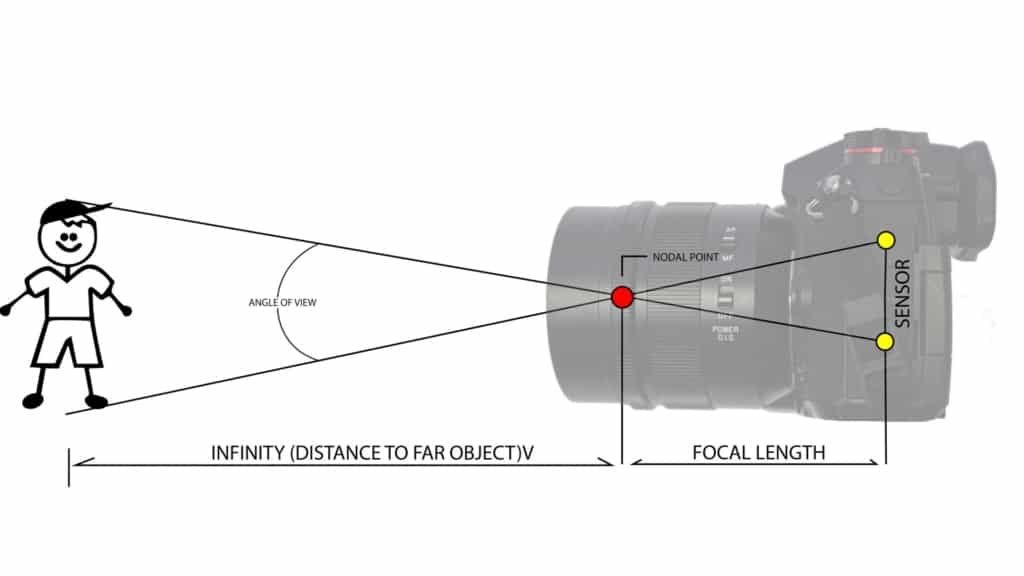
\includegraphics[width=0.8\linewidth]{figures/focal.jpg}
     \caption{Focal Length}
     \label{fig:enter-label}
 \end{figure}

\subsection{Матрица камеры (Image sensor)}
 An image sensor refers to the electronic component in a digital camera that captures and converts light into digital signals, ultimately creating a digital image. The image sensor plays a crucial role in digital photography by replacing the traditional film used in film cameras. $U=(u_1,u_2)$ - sensor size of a camera in pixels represents number of pixels along $x$ and $y$ axes respectively, total image might have upmost $u_1*u_2$ pixels, given that photo is RGB, it can be calculated, that on an 3-dimensional tensor with shape $(u_1, u_2, 3)$ the whole image can be stored, and on 4-dimensional tensor with shape $(u_1, u_2, 3, \textbf{frames})$ a whole video may be stored frome such camera without audio-stream, where frames - is the amount of frames taken from that camera consequently.



\subsection{Угловая Скорость (Angular Velocity)}
An angular velocity is the speed of rotation for an object that can be stated as ${\displaystyle \omega ={\frac {d\varphi }{dt}}}$.

\subsection{Угол Места; Элевация (Elevation)}
Vertical angle of an observed object over true horizon. Elevation combined with azimuth are used for obtaining the direction to an object. \href{https://ru.wikipedia.org/wiki/%D0%A3%D0%B3%D0%BE%D0%BB_%D0%BC%D0%B5%D1%81%D1%82%D0%B0}{Elevation}

\subsection{Азимут (Azimuth)}
Horizontal angle evaluated from predefined direction (for example north) and direction of an observed object.

\section{Простейшая задача управления камерой высокого разрешения}

Необходимо предложить алгоритм обхода всех игроков на поле начиная с центра поля.

В результате мы должны получить:

$\vec \psi(t)$ - вектор, описывающий угол места и азимут визирования камеры, как функцию времени. 

При этом мы должны обеспечить получение изображения игрока в поле зрения камеры в течение времени $\Delta T$ соответствующего $R$ кадрам. 

Движение игроков считаем априорно неизвестным. 

1) Первый шаг - обход неподвижных игроков

2) Второй шаг - обход движущихся игроков 

\subsection{Обход неподвижных игроков}

Дан взвешенный граф $G = (V, E)$, в нашем случае полный, поскольку от любой вершины может быть рационально перейти к другой, в общем случае, где

$V$ - количество распознанных на кадре объектов, на данном этапе футболистов, $V = {1, 2, 3, ..., k}$

$E$ - ребра данного графа; 

$d_{ij}(i, j \in V, i \neq j)$ - расстояние между двумя вершинами $i, j$, причем $d_{ij} > 0$,  $d_{ij} \neq \infty$ и $d_{ij} = d_{ji}$.

Требуется найти такой гамильтонов цикл (замкнутый путь), что 
\begin{align}
    minD  = \sum_{i,j \in V} d_{ij} * x_{ij},
\end{align}
где 
\begin{equation}
    x_{ij} = 
    \begin{cases}
        1 & e_{ij} \in \text{оптимальный путь}\\
        0 & e_{ij} \notin \text{оптимальный путь}
    \end{cases}
\end{equation}
То есть $x_{ij}$ - это логическая переменная, обращающаяся в 1, если ребро $e_{ij}$ удовлетворяет условию принадлежности оптимальному пути, и 0 иначе. Начало и конец обхода, в общем случае, происходят в центре футбольного поля. Результатом работы алгоритма должен быть путь, содержащий в себе все вершины графа и удовлетворяющий условиям, заданным выше.

\section{Приближения и ограничения}
 
Перемещение угла камеры вверх/вниз влево/право и фокусировка не зависят друг от друга и могут выполняться параллельно. (От этого зависит метрика оптимизируемая)

 
Мы планируем иметь количество объектов другое и сильно большее, чем количество футболистов. (От этого зависит выбор алгоритма - так как задача NP трудная то для малого количества её можно решать в лоб - гипотеза на 22 в лоб оптимальнее)

Камера должна возвращаться в исходную точку (по умолчанию - в центр). 

 
Считать что скорость бега футболиста пренебрежимо мала относительно скорости камеры нельзя.  


\chapter{Формализованная постановка задачи}
\label{cha:Proposal}
  
 \section{Задача обхода множества подвижных точек на поверхности}

{\color{red} Обращаю внимание что это не совсем задача описанная в статье - тут ребра графа меняются взаимосвязанным образом и корректно говорить все таки о задаче в ее первозданном виде.Необходимо тут сформулировать задачу в терминах поиска пути на графе заданного множеством вершин $A$ с длиной ребер вычисляемой, как функция времени. 

И хорошо бы картинками все проиллюстрировать в eps формате}


Пусть $\mathbb{R}^{3}$ - это векторное пространство, а $P_{t}$ = $\{ (x_{1}^{(t)},y_{1}^{(t)}, i_1^{(t)}), \dots,(x_{n}^{(t)},y_{n}^{(t)},i_n^{(t)}) \}$ будет набором наблюдаемых объектов, существующих в этом векторном пространстве, которые расположены на плоскости $z=0$ в момент времени $t \, \in \, \mathbb{N}$. $i \, \in \, \{0,1\}$ определяет, был ли обозрен данный объект в период $t_s < t$ ($x,y \, \in \, \mathbb{R}$). Пусть $\mathcal{P}$
$$\mathcal{P}_{t}(\hat{x}, \hat{y}, \hat{z}, \phi_{t}, \psi_{t}, z_{t},) \to \mathcal{V}$$
будет функцией проекции, которая вычисляет угловые точки проекции поля зрения $\mathcal{V}_{t}$ $\, \in \, \mathbb{R}^{{3\times4}}$ на $z=0$ в момент времени $t$. Здесь $\hat{x}, \hat{y}, \hat{z}$ - координаты камеры, $\phi_{t}, \psi_{t}, \theta_{t}, z_t$,  - тангаж, крен и zoom в момент времени $t$ (угловые координаты поворота).
%% и $\zeta$ - это коэффициент масштабирования.  %%

Пусть $\mathcal{C}$
$$
\mathcal{C}(P_{t}, \mathcal{V}_{t}) \to \begin{bmatrix}
\Delta\phi_{t}  &  \Delta\psi_{t}  &  \Delta z_t
\end{bmatrix}^{T}
$$
будет функцией контроллера, которая принимает решение о управлении направлением камеры и масштабированием для момента времени $t+1$. Вращения камеры затем обновляются следующим образом:
$$
\begin{bmatrix}
\phi_{t+1}   \\
 \psi_{t+1} \\
  z_{t+1} 
\end{bmatrix} = 
\begin{bmatrix}
\phi_{t}   \\
 \psi_{t} \\
  z_{t}
\end{bmatrix} + 
\begin{bmatrix}
\Delta\phi_{t}  \\
 \Delta\psi_{t}  \\
 \Delta z_{t}
\end{bmatrix}
$$

Пусть $\mathcal{I}$ 
$$
\mathcal{I}_{t}(\mathcal{P_{t}}, \mathcal{V}_{t}, p_{1}, p_{2}) \to a \, \in \, \{ 0,1 \}
$$
будет функцией индикатора, определяющей, занимает ли наблюдаемый объект определенную часть пространства на видоискателе и никогда не наблюдался в правильном соотношении ранее ($p_{1} \leq p \leq p2$). $a$ в этом случае является индикатором (Истина или Ложь).

Тогда ограниченная задача оптимизации выглядит следующим образом:
$$
\begin{cases}
\sum\limits_{t=1}^{T} \mathcal{I}_{t}(\mathcal{P_{t}}, \mathcal{V}_{t}, p_{1}, p_{2}) \geq n \\
T \to \min\limits_{\mathcal{C}}
\end{cases}
$$

\section{Альтернативная постановка DTSP в общем случае}
DTSP определен на полном двунаправленном графе $ G = (V, E) $, где $ V $ - это множество вершин размера $ n $, а $ E $ - множество ребер. $ V $ состоит из депо 0 и набора потенциальных агентов. Мы рассматриваем асимметричное расстояние в DTSP. Таким образом, $ E $ включает ребра в обе стороны. Агенты, которых нужно посетить, помещаются в пул агентов $ C $ размером $ c $, где $ C $ является подмножеством $ V $.

Продавец начинает свое путешествие из депо 0 в начале времени (t = 0). Он должен обслужить каждого агента в пуле $ C $ ровно один раз и затем вернуться в депо. Время путешествия от вершины $ i $ к вершине $ j $ зависит от временно-зависимой функции $ g_{ij} (t) $, где $ t $ - это время посещения вершины $ i $. Мы предполагаем, что продавец не ждет на вершине. Это верно, когда соблюдается ограничение FIFO (First-In–First-Out), то есть гарантируется, что если транспортное средство покидает вершину $ i $ для вершины $ j $ в определенное время, любое идентичное транспортное средство, покидающее вершину $ i $ для вершины $ j $ в более позднее время, прибудет позже в вершину $ j $.

Пусть $ x_{ij} $ будет бинарной решающей переменной, которая равна 1, если продавец путешествует от вершины $ i $ к вершине $ j $, и 0 в противном случае.

Пусть $ s_i $ будет временем, когда продавец посещает вершину $ i $. Цель состоит в минимизации общего времени путешествия для посещения всех агентов, то есть

$$
\min_{}\sum_{i \, \in \, \{ 0 \}\cup C}\;\sum_{j \, \in \, \{ 0 \}\cup C} g_{ij}(s_{i})x_{ij}
$$

Набор ограничений:


\begin{align}
\sum_{j \, \in \, \{ 0 \}\cup C} x_{ij} = 1 \quad  \forall i \, \in \, C \\
\sum_{i \, \in \, \{ 0 \}\cup C} x_{ji} =1 \quad  \forall i \, \in \, C \\
s_{0} = 0 \\
s_{i} + g_{ij}(s_{i})x_{ij} = s_{i} + (s_{j}-s_{i})x_{ij} \\
\forall i \, \in \, \{ 0 \} \cup C, j \, \in \, C \\
x_{ij} \, \in \, \{ 0,1 \} 
\end{align}


Ограничения (2) и (3) обеспечивают, что существует только одна входящая и исходящая вершина для агента $ i $. Ограничение (4) является начальным временем комми-вояжера в депо. Ограничения (5) указывают, что время посещения агента $ j $ зависит от времени посещения его предшественника $ i $. Этот набор ограничений также гарантирует, что время посещения на каждой вершине увеличивается вдоль пути (при условии, что $ g_{ij}(t)>0 $). Следовательно, в решении не существует подцикла.

Модель, выраженная формулами (1)–(6), по существу является формулировкой TDTSP. Она является нелинейной из-за временно-зависимой функции $ g_{ij} (t) $. Некоторые исследователи пытаются линеаризовать формулировку, накладывая дополнительные предположения. В отличие от них, в этой формулировке описывается наиболее обобщенная версию. Обратите внимание, что область $ g_{ij}(t) $ является непрерывной. Для удобства сбора данных временное пространство можно дискретизировать в набор $ T $ временных шагов. Таким образом, мы имеем время путешествия от вершины $ i $ к вершине $ j $ вокруг временного шага $ t \in T $ в качестве входных значений, обозначенных как $ d_{ij}(t) $. Здесь мы называем $ [d_{ij}(t)] $ трафиковым паттерном графа $ G $. Затем мы можем приблизить $ d_{ij}(t) $, работая с $ d_{ijt} $.

TDTSP предполагает, что все условия динамики графа известны заранее. На практике, чтобы справиться с динамической средой, мы вводим стохастическую переменную $ \phi_{ij}(t) $ в дополнение к $ g_{ij}(t) $, чтобы решить проблему неопределенности реального времени движения. Тогда фактическое время путешествия от вершины $ i $ к вершине $ j $ в момент времени $ t $, обозначенное как $ f_{ij}(t) $, равно $ f_{ij}(t) = g_{ij}(t) + \phi_{ij}(t) $. 

Чтобы решить другую проблему неопределенности, то есть изменение запросов агентов в динамической среде, мы вводим случайную операцию $ \Omega_{k} $ после того, как камера завершает осмотр $ k $-го агента, обозначенную как

$$
\Omega_{k} = \begin{cases}
1 , & \text{вставить не посещенного агента $ i $ в множество $ C $} \\
0 , & \text{ничего не делать} \\
-1,  & \text{удалить агента $ i $ из множества $ C $}
\end{cases}
$$

DTSP - это задача онлайн-оптимизации. Решить ее эффективно очень сложно. Принимая во внимание проблему масштабирования $ n = 40 $ графа G с инвариантным расположением. Если $ c = 20 $, то количество возможных экземпляров также огромно. Когда учитываются два упомянутых выше динамических аспекта, задача становится еще более сложной.      
 



\chapter{Обзор  литературы }
 
{\color{red}  В этом разделе собираем ссылки и обзор литературы по своей теме диплома. Текст - просто машинный перевод аннотаций - необходимо полностью творчески переосмыслить }

{\color{blue}  
In the article  \cite{Tinos2015} the dynamic TSP with weight changes is investigated. The effects of the changes on the fitness landscapes of the problem are analyzed. Questions regarding the dynamic TSP, like "how many solutions are affected by a change?" and "how does the severity of the problem influence the optima?", are discussed. 

Simulations of the dynamic TSP with weight changes are presented and analyzed. In the simulations, it is possible to observe that the new best solutions after a change are generally not far from the old best solutions. 


The article \cite{10.1007/11903697_31}   proposes an effective algorithm to solve DTSP. Experiments showed that this algorithm is effective, as it can find very high quality solutions using only a very short time step.
}

In the article \cite{Gharehchopogh2012} ... 


\section{Список Обозреваемой Литературы}
\begin{enumerate}
    \item \href{https://www.youtube.com/watch?v=zjMuIxRvygQ&pp=ygULcXVhdGVybmlvbnM%3D}{Quaternions and 3d rotation, explained interactively}
    \item \href{https://www.youtube.com/watch?v=d4EgbgTm0Bg&pp=ygULcXVhdGVybmlvbnM%3D}{Visualizing quaternions (4d numbers) with stereographic projection}
    \item \href{https://distill.pub/2021/gnn-intro/}{
    A Gentle Introduction to Graph Neural Networks
    }
    \item \href{https://pubmed.ncbi.nlm.nih.gov/34520362/}{
    Solving Dynamic Traveling Salesman Problems With Deep Reinforcement Learning 
    }
    \item \href{}{M. Mavrovouniotis and S. Yang, “Ant colony optimization algorithms
with immigrants schemes for the dynamic travelling salesman prob-
lem,” in Evolutionary Computation for Dynamic Optimization Problems.
Berlin, Germany: Springer, 2013, pp. 317–341} (Мета-Эвристика)
    \item \href{}{S. Jiang and S. Yang, “A benchmark generator for dynamic multi-
objective optimization problems,” in Proc. 14th UK Workshop Comput.
Intell. (UKCI), Sep. 2014, pp. 1–8.} (Мета-Эвристика)
    \item \href{}{ C. Groba, A. Sartal, and X. H. Vázquez, “Solving the dynamic traveling
salesman problem using a genetic algorithm with trajectory prediction:
An application to fish aggregating devices,” Comput. Oper. Res., vol. 56,
pp. 22–32, Apr. 2015.} (Мета-Эвристика)
    \item \href{}{J.-F. Cordeau, G. Ghiani, and E. Guerriero, “Analysis and branch-and-cut
algorithm for the time-dependent travelling salesman problem,” Transp.
Sci., vol. 48, no. 1, pp. 46–58, Feb. 2014} (Linearization of TDTSP)
    \item \href{}{A. Montero, I. Méndez-Díaz, and J. J. Miranda-Bront, “An integer
programming approach for the time-dependent traveling salesman prob-
lem with time Windows,” Comput. Oper. Res., vol. 88, pp. 280–289,
Dec. 2017.} (Linearization of TDTSP)
    \item \href{https://cnrrobertson.github.io/other/mlseminar/fall_2021/Stochastic%20Temporal%20Networks%20-%20Binan%20Gu.pdf}{Stochastic Temporal Networks}
    \item \href{https://towardsdatascience.com/temporal-graph-learning-in-2024-feaa9371b8e2}{Temporal Graph Learning in 2024}
    \item \href{https://link.springer.com/book/10.1007/b101971}{The Traveling Salesman Problem and Its Variations}
    \item \href{https://www.sciencedirect.com/science/article/pii/S1572528608000339}{The time-dependent traveling salesman problem and single machine
scheduling problems with sequence dependent setup times
Louis-Philippe Bigras, Michel Gamache, Gilles Savard} (Очень похожая постановка задачи)
    \item \href{https://arxiv.org/abs/1803.08475}{W. Kool, H. Van Hoof, and M. Welling, “Attention, learn to solve routing
problems!,” in Proc. Int. Conf. Learn. Represent., 2019.}
    \item \href{https://medium.com/stanford-cs224w/tackling-the-traveling-salesman-problem-with-graph-neural-networks-b86ef4300c6e}{Tackling the Traveling Salesman Problem with Graph Neural Networks}
\end{enumerate}

\section{Описание Релевантных Идей}

\subsection{Temporal Graphs (Временные Графы)}

$\bullet$ Each edge $e = (u, v, t) \in E$ is a temporal edge from a vertex $u$ to another vertex $v$ at time $t$ . For any two temporal ages $(u,v,t_1)$ and $(u,v,t_2)$ $t_1 \neq t_2$.

$\bullet$ Each vertex v $\in$ V is active when there is a temporal edge that starts or ends at v.

$\bullet$ d(u, v): the number of temporal edges from u to v in G.

$ \bullet $ E(u, v): the set of temporal edges from u to v in G,  i.e, $E(u,v)=\{(u,v,t_1),(u,v,t_2), ..., (u,v,t_{d(u,v)} )\}$

$\bullet$ $N_{out}(v)$ or $N_{in} (v)$: the set of out-neighbors or in-neighbors
of $v$ in $G$, i.e., $N_{out}(v) = \{u : (v, u, t) ∈ E\}$ and $N_{in}(v) =
\{u : (u, v, t) ∈ E\}$.

$\bullet$ $d_{out}(v)$ or $d_{in} (v)$: the temporal out-degree or in-degree of v
in G, defined as $d_{out}(v) = \sum_{u \in N_{out(v}} d(v,u)$ and $d_{in} (v) = sum_{u \in N_{in(v}}d(u,v)$

\subsection{Подвиды TSP}
Опираясь на книгу The Traveling Salesman Problem and Its Variations, в глаза бросаются две разновидности TSP, которые кажутся наиболее актуальными для нашей проблемы:


{\color{blue}
Moving Target TSP: A set $X = \{x_1, x_2, \ldots, x_n\}$ of $n$ objects placed at points $\{p_1, p_2, \ldots, p_n\}$. Each object $x_i$ is moving from $p_i \in \mathbb{R}^2$ at velocity $v_i$. A pursuer starting at the origin moving with speed $v$ wants to intercept all points $x_1, x_2, \ldots, x_n$ in the fastest possible time. This problem is related to the time-dependent TSP.




Time-Dependent TSP: For each arc $(i, j)$ of $G$, $n$ different costs $c_{ij}^t = 1, 2, \ldots, n$ are given. The cost $c_{ij}^t$ corresponds to the 'cost' of going from city $i$ to city $j$ in time period $t$. The objective is to find a tour $(\tau(1), \tau(2), \ldots, \tau(n), \tau(1))$, where $\tau(1) = 1$ corresponds to the home location which is in time period zero, in $G$ such that $\sum_{i=1}^{n} c_{\tau(i) \tau(i+1)}^{t_i}$ is minimized. The index $n + 1$ is equivalent to 1. For all $(i, j)$, if $c_{ij}^t = c_{ji}^t = \ldots = c_{ij}^{t'}$, then the time-dependent TSP reduces to the traveling salesman problem.

}

В нашем случае, кажется, что проблема вбирает в себя оба подвида.

\subsection{Глубинное Обучение с Подкреплением}
В 2023 году была опубликована статья \cite{RL}, формулирующая задачу, сходную с рассматриваемой в данной работе. Оказалось, что рассматриваемая нами задача скорее относится к Time-Dependent TSP (TDTSP), а не к Dynamic TSP (DTSP), как изначально предполагалось. Авторы использовали подход Deep Reinforcement Learning для решения этой задачи, вводя дополнительное усложнение: новые вершины могут исчезать и появляться в процессе, что, в свою очередь, может быть актуально и для футбольного поля. При условии решения проблемы с данными (обеспечение достаточного объема данных для обучения RL модели с механизмом внимания), методика авторов статьи может быть адаптирована под наш случай.

\subsection{Проблема Маршрутизации Транспорта (Vehicle Routing Problem)}

Постановка задачи VRP:
Задача маршрутизации транспортных средств (VRP) представляет собой оптимизационную задачу, целью которой является нахождение оптимальных маршрутов для флота транспортных средств с учетом нескольких факторов, таких как время, стоимость и грузоподъемность. Формально, в VRP имеется заданное количество транспортных средств, каждое из которых имеет ограничения по грузоподъемности и времени работы. Также имеется набор клиентских точек, которые необходимо посетить, и для каждой точки известны требования по грузу и времени обслуживания. Целью VRP является оптимальное распределение клиентских точек между транспортными средствами таким образом, чтобы минимизировать общие затраты, учитывая все ограничения.

Отличие от TSP:
Главное отличие между TSP и VRP заключается в том, что в TSP имеется один продавец, который должен посетить набор городов и вернуться в исходную точку, минимизируя общее расстояние, в то время как в VRP есть несколько транспортных средств, каждое из которых должно обслужить набор клиентских точек с определенными ограничениями. Таким образом, в VRP необходимо оптимизировать распределение клиентских точек между транспортными средствами с учетом различных факторов, включая грузоподъемность, время обслуживания и пропускную способность, что делает эту задачу более сложной по сравнению с TSP. VRP постановка пробелмы может быть актуальна в случае с несколькими наблюдающими камерами.

\subsection{CGN (Convolutional Graph Networks) для TSP}
 В статье \cite{gnn} рассматривается использование GNN для оптимизации маршрута в условиях, когда необходимо посетить множество городов и вернуться в исходный пункт. Обсуждаются основы проблемы, применение GNN к ней, а также детали реализации модели с использованием Graph Transformer и Residual Gated GCN. В заключении отмечается, что модель демонстрирует способность находить оптимальные маршруты, но требует размеченных данных, и перспективным направлением развития может быть переход к обучению с подкреплением. Размеченные данные получаются при помощи Concorde TSP Solver, то есть сначала нужно посчитать оптимальные пути для графов, а потом начать обучать нейронную сеть. 
   
 
\chapter{Описание решения}
 {\color{red} Это раздел для декомпозиции задачи и описание Methods для каждой подзадачи   }

 \section{Используемые системы координат   }\label{41}
На данном этапе используются две системы координат: 1-я, связанная с футбольным полем, где левый верхний угол считается точкой (0, 0) и 2-я, связанная с координатами камеры, в системе отсчета, связанной с левым дальним углом поля. Для наперед заданных координат  $X,\;Y$ переход от одной плоскости к другой осуществляется по нижеследующему закону:

$$
\begin{bmatrix}
\tau_{i}X' \\
\tau_{i}Y' \\
\tau_{i}
\end{bmatrix} = 
\underbrace{ \begin{bmatrix}
a_{1} & a_{2} & b_{1} \\
a_{3} & a_{4} & b_{2} \\
c_{1} & c_{2} & 1
\end{bmatrix} }_{ M } \begin{bmatrix}
X \\
Y \\
1
\end{bmatrix},
$$

где $a_i$ это элементы масштабирования/поворота, $\begin{bmatrix}
    b_2 & b_1
\end{bmatrix}^T$ это вектор смещения и $\begin{bmatrix}
    c_1 & c_2
\end{bmatrix}$ это вектор проекции.

Для нахождения истинных значений $X', Y'$ результирующий вектор должен быть поделен на коэффициент $\tau_i$, который является фактором масштабирования. 

В результате был разработан алгоритм, с использованием библиотеки cv2, который принимает на вход 2 аргумента, а именно 4 первоначальные координаты (x, y), которые показывают первоначальные углы прямоугольника захватываемой для перехода области, а также второй аргумент - 4 координаты, которые показывают желаемые угловые координаты для выходной картинки. В результате работы алгоритма получена матрица перехода $M \in \mathbb{R}^{3 \times 3}$, после чего алгоритм последовательно применяется к каждому отдельно взятому кадру из изначально заданного набора данных. В результате, получается новый набор данных, в котором для каждого id, то есть распознанного на кадре объекта, получены новые координаты ($X', Y'$). Пример, визуализирующий работу алгоритма:

 \begin{figure}[!h]
     \centering
     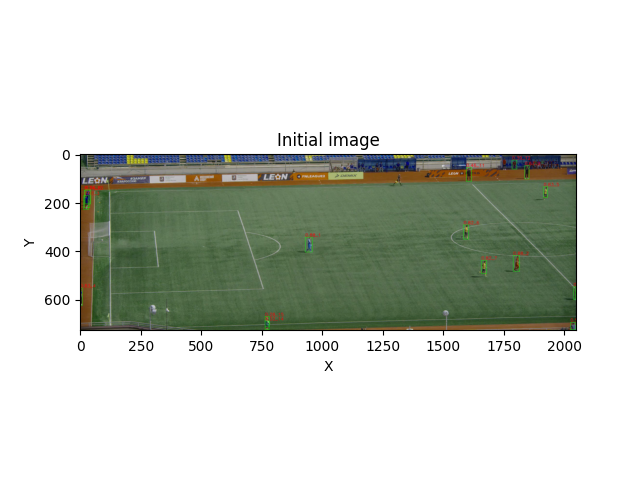
\includegraphics[width=0.8\linewidth]{figures/Initial image.png}
     \caption{Image before transformation of coordinates}
     \label{fig:before-transform}
 \end{figure}

  \begin{figure}[!h]
     \centering
     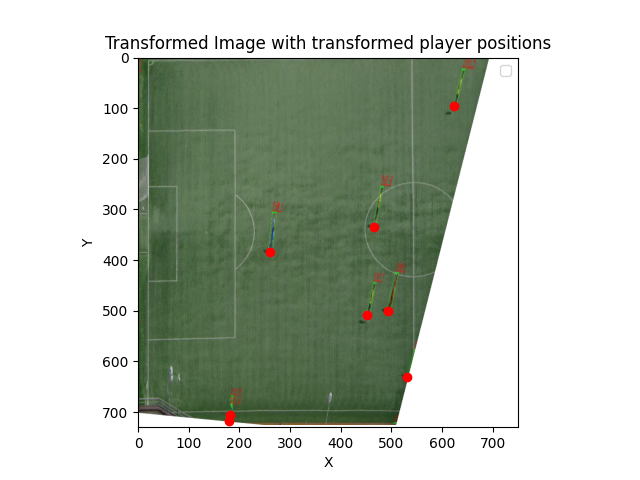
\includegraphics[width=0.8\linewidth]{figures/Transformed Image with transformed player positions.png}
     \caption{Image after transformation of coordinates}
     \label{fig:after-transform}
 \end{figure}


 \section{Предварительная обработка}

 \section{Разработка алгоритма обхода для случая неподвижных игроков   }
Для решения задачи TSP существует множество решений, однако между ними есть ряд ключевых отличий, основным из которых является точность решения. Есть алгоритмы, способные решить задачу нахождения минимального замкнутого пути точно, есть те, что не гарантируют минимальный обход, однако значительно выигрывают в скорости. Для данной конкретной задачи был выбран вариант точного решения, поскольку количество n, то есть количество распознанных на кадре объектов невелико.

Таким образом, согласно статье~\cite{Zhang_2021} наиболее оптимальным вариантом оказался dynamic programming method, поскольку среди точных подходов к решению TSP он показал наибольшую скорость. Реализованный алгоритм принимает на вход один кадр с распознанными объектами, с уже трансформированными координатами, переход к которым был решен в пункте \ref{41}, и возвращает путь, включающий в себя id всех распознанных на кадре объектов, в порядке, который позволяет минимизировать гамильтонов замкнутый путь на графе, вершинами которого являются id, а также сумму пути. Для следующей задачи разработки алгоритма обхода для случая подвижных игроков, вероятно, придется пересмотреть алгоритмический подход к решению задачи, тем не менее dynamic programming подход можно считать успешным на текущем этапе. 

\section{Симуляция Среды}
\subsection{Симуляция агентов}
\subsection{Симуляция камеры}
Пересечение плоскости с прямой:
Пусть $p_0$ - это вектор камеры, а $v_0$ - вектор направления света угловой точки фокальной плоскости, проходящий через вектор камеры (центр фокусного объектива).

Тогда параметрическое уравнение прямой может быть определено как:
$$P(t) = p_0 + t \cdot v_0 \qquad \text{($P(t)$ - точка на прямой)}$$

Нам нужно найти такое $t$, что $P(t)$ лежит на заданной плоскости.
Подставив это в уравнение плоскости, мы получаем:
$$a(P0_x + tV0_x) + b(P0_y + tV0_y) + c(P0_z + tV0_z) = d$$

Решая для $t$ ($n$ - нормальный вектор плоскости):
$$t = \frac{D - nP0}{n \cdot V0}$$

Нас интересует $t < 0$, так как положительные значения соответствуют неправильному направлению света.

\subsubsection{Поле зрения и угол зрения}
Поле зрения:  Метод calculatePanoramicSystemFOV вычисляет угол обзора (FOV) для каждой камеры в
панорамной системе и возвращает список углов обзора камер для панорамной системы.

Метод определяет вектор плоскости и координаты и углы поворота панорамной системы. Затем для каждой камеры в панорамной системе происходит следующее:

    \begin{enumerate}
        \item Вычисляются координаты камеры и ее углы обзора.
        \item Создаются векторы, определяющие углы обзора камеры.
        \item Применяются повороты к векторам камеры и панорамной системы.
        \item Рассчитывается точка пересечения прямой (определяемой камерой) с плоскостью (панорамной системой).
        \item Вычисляется угол обзора камеры и основная ось обзора камеры.
    \end{enumerate}


1. Вычисление вектора vector a:
$$
\text{vector\_a} = \begin{bmatrix}
1.0 \\
\tan\left(\frac{\text{camera\_width\_angle\_of\_view}}{2}\right) \\
-\tan\left(\frac{\text{camera\_height\_angle\_of\_view}}{2}\right)
\end{bmatrix}
$$

2. Поворот вектора $ \mathbf{a} $:
$$
\mathbf{a} = \left(\mathbf{R}_\text{ps} \cdot \mathbf{R}_\text{c}\right) \cdot \mathbf{a}
$$

Здесь $ \mathbf{R}_\text{ps} $ и $ \mathbf{R}_\text{c} $ представляют собой матрицы поворота для панорамной системы и камеры соответственно.

3. Повторный поворот векторов $ \mathbf{b} $, $ \mathbf{c} $, $ \mathbf{d} $, $ \mathbf{p} $:
\begin{align*}
\mathbf{b} &= \left(\mathbf{R}_\text{ps} \cdot \mathbf{R}_\text{c}\right) \cdot \mathbf{b} \\
\mathbf{c} &= \left(\mathbf{R}_\text{ps} \cdot \mathbf{R}_\text{c}\right) \cdot \mathbf{c} \\
\mathbf{d} &= \left(\mathbf{R}_\text{ps} \cdot \mathbf{R}_\text{c}\right) \cdot \mathbf{d} \\
\mathbf{p} &= \left(\mathbf{R}_\text{ps} \cdot \mathbf{R}_\text{c}\right) \cdot \mathbf{p} 
\end{align*}

Здесь $ \mathbf{R}_\text{ps} $ и $ \mathbf{R}_\text{c} $ также представляют собой матрицы поворота для панорамной системы и камеры.

4. Вычисление точки $ \mathbf{t}_0 $:
$$
\mathbf{t}_0 = \mathbf{r}_\text{ps} + \mathbf{R}_\text{ps} \cdot \mathbf{r}_\text{c}
$$

Здесь $ \mathbf{r}_\text{ps} $ и $ \mathbf{r}_\text{c} $ представляют собой координаты панорамной системы и камеры соответственно.
5. Определение параметров $a_0$, $b_0$, $c_0$, $d_0$, $p_0$:

\begin{align*}
a_0 &= -\frac{\left(\mathbf{v}_\text{plane} \cdot \mathbf{v}_{\text{t}_0}\right) + D} {\left(\mathbf{v}_\text{plane} \cdot \mathbf{v}_a\right)} \\
b_0 &= -\frac{\left(\mathbf{v}_\text{plane} \cdot \mathbf{v}_{\text{t}_0}\right) + D} {\left(\mathbf{v}_\text{plane} \cdot \mathbf{v}_b\right)} \\
c_0 &= -\frac{\left(\mathbf{v}_\text{plane} \cdot \mathbf{v}_{\text{t}_0}\right) + D}{\left(\mathbf{v}_\text{plane} \cdot \mathbf{v}_c\right)} \\
d_0 &= -\frac{\left(\mathbf{v}_\text{plane} \cdot \mathbf{v}_{\text{t}_0}\right) + D}{\left(\mathbf{v}_\text{plane} \cdot \mathbf{v}_d\right)} \\
p_0 &= -\frac{\left(\mathbf{v}_\text{plane} \cdot \mathbf{v}_{\text{t}_0}\right) + D}{\left(\mathbf{v}_\text{plane} \cdot \mathbf{v}_p\right)}
\end{align*}

6. Расчет координат углов обзора и основной оси камеры:
\begin{align*}
\text{fov\_a} &= a_0 \cdot \mathbf{v}_a + \mathbf{v}_{\text{t}_0} \\
\text{fov\_b} &= b_0 \cdot \mathbf{v}_b + \mathbf{v}_{\text{t}_0} \\ 
\text{fov\_c} &= c_0 \cdot \mathbf{v}_c + \mathbf{v}_{\text{t}_0} \\ 
\text{fov\_d} &= d_0 \cdot \mathbf{v}_d + \mathbf{v}_{\text{t}_0} \\ 
\text{main\_axis} &= p_0 \cdot \mathbf{v}_p + \mathbf{v}_{\text{t}_0} \\
\end{align*}

Эти преобразования необходимы для вычисления параметров углов обзора и основной оси камеры в панорамной системе. Они осуществляют преобразования координат и векторов, учитывая их начальные положения и повороты относительно системы координат, связанных с панорамной системой. Затем, используя найденные параметры, определяются точки, обозначающие углы обзора каждой камеры, а также точка, представляющая основную ось камеры. Эти шаги позволяют определить положение и направление обзора каждой камеры в контексте панорамной системы.


Угол зрения (Angle of View): 
Этот метод вычисляет вертикальный угол обзора камеры. Рассмотрим математику этого процесса.

Пусть $f$ - фокусное расстояние объектива камеры, $H$ - высота фокальной плоскости камеры. Мы хотим найти вертикальный угол обзора $\theta_{\text{vertical}}$, который позволяет определить, сколько градусов по вертикали охватывает камера.

Используя теорему о подобных треугольниках, мы понимаем, что вертикальный угол обзора можно выразить как двойной арктангенс отношения высоты фокальной плоскости к удвоенному фокусному расстояния:

$$
\theta_{\text{vertical}} = 2 \times \arctan \left( \frac{H}{2f} \right)
$$

Таким образом, мы находим угол, под которым видно изображение на фокальной плоскости относительно центральной оси камеры. Это дает нам представление о том, какая часть вертикального пространства охватывается изображением.

\subsubsection{Определение $\Delta$ крен и $\Delta$ тангаж в процессе перемещения}
Для симуляции камеры и алгоритма в целом важно иметь возможность управлять камерой. 
Для того, чтобы управлять камерой, в нашем исследовании, мы можем отправлять $\Delta \theta$  и $\Delta \phi$ ($\Delta$ крен и $\Delta$ тангаж) изменения в нашу камеру (симулируемую либо реальную). 


1. Центральная точка углов обзора:

   Находим центральную точку между двумя угловыми точками обзора (FOV):

   Пусть  $ P_1  $ и  $ P_2  $ - две угловые точки обзора камеры, тогда центральная точка  $ C  $ будет:

    $$
   C = \left( \frac{P_{1x} + P_{2x}}{2}, \frac{P_{1y} + P_{2y}}{2} \right)
    $$

2. Вычисление угла:

   Рассчитываем угол наклона камеры относительно горизонтали и вертикальный угол обзора камеры:

   Пусть  $ (x_c, y_c)  $ - координаты камеры,  $ (x_i, y_i)  $ - начальная позиция,  $ (x_t, y_t)  $ - целевая позиция. Также  $ h  $ - высота камеры, а  $ \theta_{\text{pitch}}  $ - угол вертикального обзора, $\theta_0$ - угол вертикального наклона в данный момент, $\theta_{\text{top\_aov}}$ - угол между высшим входящим лучем света на фотокамеру и основной оси камеры ($AOV_{\text{vert}}/2$).   

   Для начала определяем угол наклона камеры (yaw), используя векторы направления от камеры к начальной и целевой позициям:

    $$
   \Delta \theta_{\text{yaw}} = \text{atan2}(y_t - y_c, x_t - x_c) - \text{atan2}(y_i - y_c, x_i - x_c)
    $$

   Затем вычисляем угол тангажа (pitch), который представляет собой угол наклона камеры относительно горизонта для:


    $$
   \theta_{\text{pitch}} = 90^\circ - \text{toDegrees}(\arctan( \frac{|(x_t-x_c, y_t-y_c) | }{h}) )
    $$

    $$
   \Delta \theta_{\text{pitch}} = \theta_{\text{pitch}} - \theta_{\text{top\_aov}} - \theta_{0}
    $$

Здесь  $ \text{atan2}  $ - функция арктангенса двух аргументов,  $ \| \cdot \|  $ - норма вектора, а  $\mod$ - операция взятия остатка от деления.




\section{Разработка алгоритма обхода для случая подвижных игроков}
 
 Движение игроков считаем априорно неизвестным. 

\subsection{Master-Route Baseline}
Базовый алгоритм, является прохождением камерой по полю *змейкой*. Камера поочередно осматривает каждую полосу наблюдаемого поля, проходя от левого края поля к правому, а затем от правого края поля к левому. Такая алгоритмика легко реализуется после того как фреймворк из секции 4.4.2 был реализован. Чтобы иплементировать обход по всем игрокам, можно приближать камеру по пути, когда алгоритм определяет, что игрок достаточно близок к его первоначальной територии.


\subsection{Probability-Density-Graphs TSP}
Предположим, что мы знаем граф игроков в момент t. Признаками вершин в такой ситуации будут координаты игроков а также идентификаторы. Обучим алгоритм, который для каждого игрока может по последовательности $[0,t]$ предсказывать вероятностное распределение его позиции (самый простой кейс - 2-мерный гауссиан, то есть стандартное нормальное распределение), тогда можно поставить целью для камеры сфокусироваться на 95\%-ом интервале уверенности в момент t+k, который можно вычислить, используя угловую скорость камеры. Далее камера наводится на вершину так, чтобы была видная вся область с достаточной уверенностью и приближается на конкретного игрока (можно включить здесь линейную интерполяцию его движения). Далее алгоритм повторяется для всех игроков.       




 \chapter{Результаты}

 
\section{Выбор и обоснование метрик для решаемой задачи }

\section{Результаты вычисления метрик для статической картинки }

\section{Результаты вычисления метрик для множества подвижных объектов }

Можно использовать Reinforcement Learning подобно Tesla, для управления камерой, создать симуляцию для обучения камеры.

Можно использовать какие-то алгоритмы для графового МЛ (\url{https://paperswithcode.com/methods/area/graphs})


%\include{6-specification}
%\section{Спецификация оборудования}

Перечень оборудования, поставленного по   Муниципальному контракту №0350300011821000371\_175478 от 04.10.2021г. на поставку серверного оборудования для подсистемы видеонаблюдения АПК «Безопасный город», серверного оборудования к существующей инфраструктуре Заказчика приведен в таблице \ref{tab:spec}.

\begin{landscape} 
\begin{center}
\begin{longtable}{|l|l|l|l|}
\caption{Спецификация оборудования поставленного по   Муниципальному контракту №0350300011821000371\_175478 от 04.10.2021г.} \label{tab:spec}  \\

\hline \multicolumn{1}{|c|}{\textbf{№}} & \multicolumn{1}{p{110pt}|}{\textbf{Наименование }} & \multicolumn{1}{p{160pt}|}{\textbf{Спецификация}}  & 
\multicolumn{1}{p{70pt}|}{\textbf{Имя и IP}} \\ \hline 
\endfirsthead

\multicolumn{4}{p{340pt}}%
{{\bfseries \tablename\ \thetable{} -- продолжение}} \\
\hline \multicolumn{1}{|c|}{\textbf{№}} & \multicolumn{1}{p{110pt}|}{\textbf{Наименование }} & \multicolumn{1}{p{160pt}|}{\textbf{Спецификация}} & 
\multicolumn{1}{p{70pt}|}{\textbf{Имя и IP}}  \\ \hline 
\endhead

\hline \multicolumn{4}{|r|}{{Продолжение на сл.странице}} \\ \hline
\endfoot

\hline \hline
\endlastfoot

1 & МВЯ -1 & Intel  i9 10900x, ddr4 32gb, sad 120gb,sfp+ 10gbit, RTX3060ti x2  & MPC01  194.255.255.0 \\\hline
2 & МВЯ -2 & Intel  i9 10900x, ddr4 32gb, sad 120gb,sfp+ 10gbit, RTX3060ti x2    & MPC02 \\\hline
3 & МХВ -1 &Intel   corei7 -9700,ОЗУ 16 Gb , 1хssd 120g+12х6тб, sfp+ 10gbit   & SS01\\\hline
4 & МХВ -2 & Intel   corei7 -9700,ОЗУ 16 Gb , 1хssd 120g+12х6тб, sfp+ 10gbit  & SS02\\\hline
5 & МХВ -3 & Intel   corei7 -9700,ОЗУ 16 Gb , 1хssd 120g+12х6тб, sfp+ 10gbit   & SS03\\\hline
6 & МХВ -4 & Intel   corei7 -9700,ОЗУ 16 Gb , 1хssd 120g+12х6тб, sfp+ 10gbit   & SS04\\\hline
7 & МХВ -5 &Intel   corei7 -9700,ОЗУ 16 Gb , 1хssd 120g+12х6тб, sfp+ 10gbit    & SS05\\\hline
8 & МХВ -6 & Intel   corei7 -9700,ОЗУ 16 Gb , 1хssd 120g+12х6тб, sfp+ 10gbit   & SS06\\\hline
9 & Коммутатор ТШ-2 & MikroTik CRS317  & MTIK317 \\\hline
10 & KVM & Aten & \\\hline
11  & Коммутатор ТШ-1  &MikroTik CRS326   & MTIK326\\\hline
12 & ИБП 10000   & IPPON 10000VA
SNMP card  & \\\hline
13  & ТШ-2   &   & \\\hline
 
\end{longtable}
\end{center}
\end{landscape}  

%\include{7-port-comm}

\backmatter %% Здесь заканчивается нумерованная часть документа и начинаются ссылки и
            %% заключение

%\chapter*{Заключение}

Разработанная  


   % Выводы 

% % Список литературы при помощи BibTeX
% Юзать так:
%
% pdflatex rpz
% bibtex rpz
% pdflatex rpz

\bibliographystyle{gost780u}
\bibliography{cam-tsp}

%%% Local Variables: 
%%% mode: latex
%%% TeX-master: "rpz"
%%% End:       % Список литературы 

%\include{98-Otzyv}

%\appendix   % Тут идут приложения

%\include{91-appendix2} 

% %\chapter*{Перечень внесенных изменений}
\Large{Лист изменений}
\small
\begin{longtable}{|p{90pt}|p{100pt}|p{260pt}|p{80pt}|}
 
\hline
\textbf{Дата} & \textbf{Автор} & \textbf{Внесенные изменения.}   \\
\hline
\endfirsthead
\multicolumn{4}{c}%
{\tablename\ \thetable\ -- \textit{Продолжение}} \\
\hline
\textbf{Дата} & \textbf{Автор} &\textbf{Внесенные изменения.}   \\
\hline
\endhead
\hline \multicolumn{4}{r}{\textit{Продолжение на следующей странице}} \\
\endfoot
\hline
\endlastfoot
  	 &   &    \\\hline
 	 &   &   \\  \hline
 	 & &    \\\hline
 	 & &    \\\hline
 	 & &    \\\hline 
 	 & &    \\\hline
 	 & &    \\\hline
 	 & &    \\\hline
 	 & &    \\\hline
 	 & &    \\\hline
 	 & &    \\\hline
 	 
\end{longtable}



\end{document}

%%% Local Variables:
%%% mode: latex
%%% TeX-master: t
%%% End:
